\documentclass{article}
\usepackage[utf8]{inputenc}
\usepackage{graphicx} % Required for inserting images
\usepackage{hyperref}
\usepackage{subcaption}
\usepackage{float}
\usepackage{tcolorbox}
\usepackage{amsmath}
\usepackage{amssymb}
\usepackage{listings}% http://ctan.org/pkg/listings}
\usepackage{algorithm}
\usepackage{algorithmic}
\usepackage[toc,page]{appendix}
%\usepackage[backend=biber]{biblatex}
\usepackage{multicol}
\usepackage{siunitx}
\usepackage{comment}
\usepackage{xcolor}
\usepackage{caption}
\usepackage{forest}
\usepackage{tikz}
\usetikzlibrary{shapes.geometric, arrows}


\tikzstyle{startstop} = [rectangle, rounded corners, 
minimum width=3cm, 
minimum height=1cm,
text centered, 
draw=black, 
fill=red!30]

\tikzstyle{io} = [trapezium, 
trapezium stretches=true, % A later addition
trapezium left angle=70, 
trapezium right angle=110, 
minimum width=3cm, 
minimum height=1cm, text centered, 
draw=black, fill=blue!30]

\tikzstyle{process} = [rectangle, 
minimum width=3cm, 
minimum height=1cm, 
text centered, 
text width=3cm, 
draw=black, 
fill=orange!30]

\tikzstyle{decision} = [diamond, 
minimum width=3cm, 
minimum height=1cm, 
text centered, 
draw=black, 
fill=green!30]
\tikzstyle{arrow} = [thick,->,>=stealth]

% To delete lstlisting caption "Listing x"
%\captionsetup[lstlisting]{labelformat=empty}

\lstdefinestyle{myStyle}{
    belowcaptionskip=1\baselineskip,
    breaklines=true,
    frame=none,
    numbers=none, 
    basicstyle=\footnotesize\ttfamily,
    keywordstyle=\bfseries\color{green!40!black},
    commentstyle=\itshape\color{purple!40!black},
    identifierstyle=\color{black},
    backgroundcolor=\color{white},
}

\lstdefinestyle{cypherStyle}{
    backgroundcolor=\color{white},   % choose the background color
    basicstyle=\footnotesize\ttfamily,        % the size of the fonts that are used for the code
    commentstyle=\itshape\color{purple!40!black},
    keywordstyle=\bfseries\color{green!40!black},
    breakatwhitespace=false,         % sets if automatic breaks should only happen at whitespace
    breaklines=true,                 % sets automatic line breaking
    captionpos=b,                    % sets the caption-position to bottom
    commentstyle=\color{gray},    % comment style
    deletekeywords={},            % if you want to delete keywords from the given language
    escapeinside={\%*}{*)},          % if you want to add LaTeX within your code
    extendedchars=true,              % lets you use non-ASCII characters; for 8-bits encodings only, does not work with UTF-8
    %firstnumber=1000,                % start line enumeration with line 1000
    frame=none,                    % adds a frame around the code
    keepspaces=true,                 % keeps spaces in text, useful for keeping indentation of code (possibly needs columns=flexible)
    language=SQL,                    % the language of the code
    morekeywords={*,IF, REQUIRE, FOR, IS, LOAD, CSV, WITH, HEADERS, MERGE, toFloat, toInteger, date},            % if you want to add more keywords to the set
    numbers=none,                    % where to put the line-numbers; possible values are (none, left, right)
    numbersep=5pt,                   % how far the line-numbers are from the code
    numberstyle=\tiny\color{mygray}, % the style that is used for the line-numbers
    rulecolor=\color{black},         % if not set, the frame-color may be changed on line-breaks within not-black text (e.g. comments (green here))
    showspaces=false,                % show spaces everywhere adding particular underscores; it overrides 'showstringspaces'
    showstringspaces=false,          % underline spaces within strings only
    showtabs=false,                  % show tabs within strings adding particular underscores
    stepnumber=1,                    % the step between two line-numbers. If it's 1, each line will be numbered
    stringstyle=\ttfamily,     % string literal style
    tabsize=2,                       % sets default tabsize to 2 spaces
}

%% Golang definition for listings
%% http://github.io/julienc91/lstlistings-golang
%%
\lstdefinelanguage{Golang}%
  {morekeywords=[1]{package,import,func,type,struct,return,defer,panic,%
     recover,select,var,const,iota,},%
   morekeywords=[2]{string,uint,uint8,uint16,uint32,uint64,int,int8,int16,%
     int32,int64,bool,float32,float64,complex64,complex128,byte,rune,uintptr,%
     error,interface},%
   morekeywords=[3]{map,slice,make,new,nil,len,cap,copy,close,true,false,%
     delete,append,real,imag,complex,chan,},%
   morekeywords=[4]{for,break,continue,range,go,goto,switch,case,fallthrough,if,%
     else,default,},%
   morekeywords=[5]{Println,Printf,Error,Print,},%
   sensitive=true,%
   morecomment=[l]{//},%
   morecomment=[s]{/*}{*/},%
   morestring=[b]',%
   morestring=[b]",%
   morestring=[s]{`}{`},%
}

\lstdefinestyle{golangStyle}{
    captionpos=b,              % sets the caption-position to bottom
    belowcaptionskip=1\baselineskip,
    breaklines=true,
    frame=none,
    numbers=none, 
    basicstyle=\footnotesize\ttfamily,
    keywordstyle=\bfseries\color{green!40!black},
    commentstyle=\itshape\color{purple!40!black},
    identifierstyle=\color{black},
    backgroundcolor=\color{white},
    language=Golang,
}


\title{TFM-FernandoMartín}
\author{Fernando Martín Canfrán}

\begin{document}

\section{Dynamic Pipeline}

\textcolor{red}{\textbf{TODO: Switch the drawings and the description, edge and event channel merged in 1 single channel}}\\

\begin{figure}[H]
    \centering
    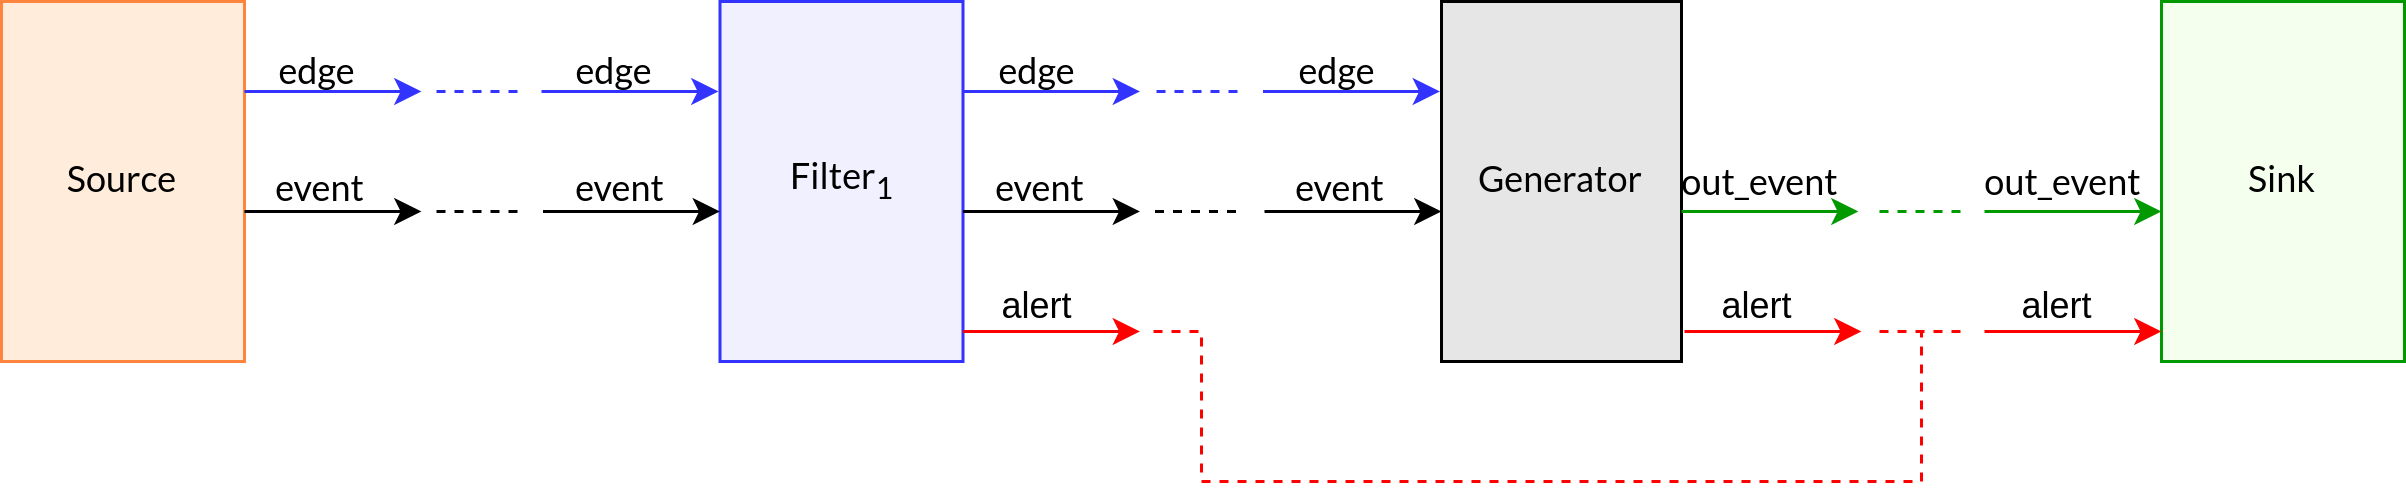
\includegraphics[scale = 0.7]{images/pipeline-schema.png}
    \caption{Pipeline Schema}
    \label{img:pipeline-schema}
\end{figure}

Description of the channels:
\begin{itemize}
    \item \texttt{edge}: only edge dedicated channel \textcolor{red}{$\rightarrow$ NO}
    \item \texttt{event}: events channel
    \item \texttt{alert}: direct channel from the filters (in particular the filter worker) to the sink (it does not go through the Generator, although it has it to be able to give it to the filters so that they are able to write on it)
    \item \texttt{out\_event}: direct dedicated event channel between Generator and Sink.
    \item \texttt{internal\_edge}: edge channel between filter and its worker. Used to communicate to the worker the edges belonging to the filter that the worker needs to process. \textcolor{red}{$\rightarrow$ Now events and not only edges, and also distinguishing between start and end edges on the type of event.}
    \item \texttt{endchan}: synchronization channel between Filter and Worker, to let Filter know whenever Worker is done. To avoid finishing the filter before the worker is actually done. \textcolor{red}{TODO: Include in the drawing}
  \end{itemize}


\begin{figure}[H]
  \centering
  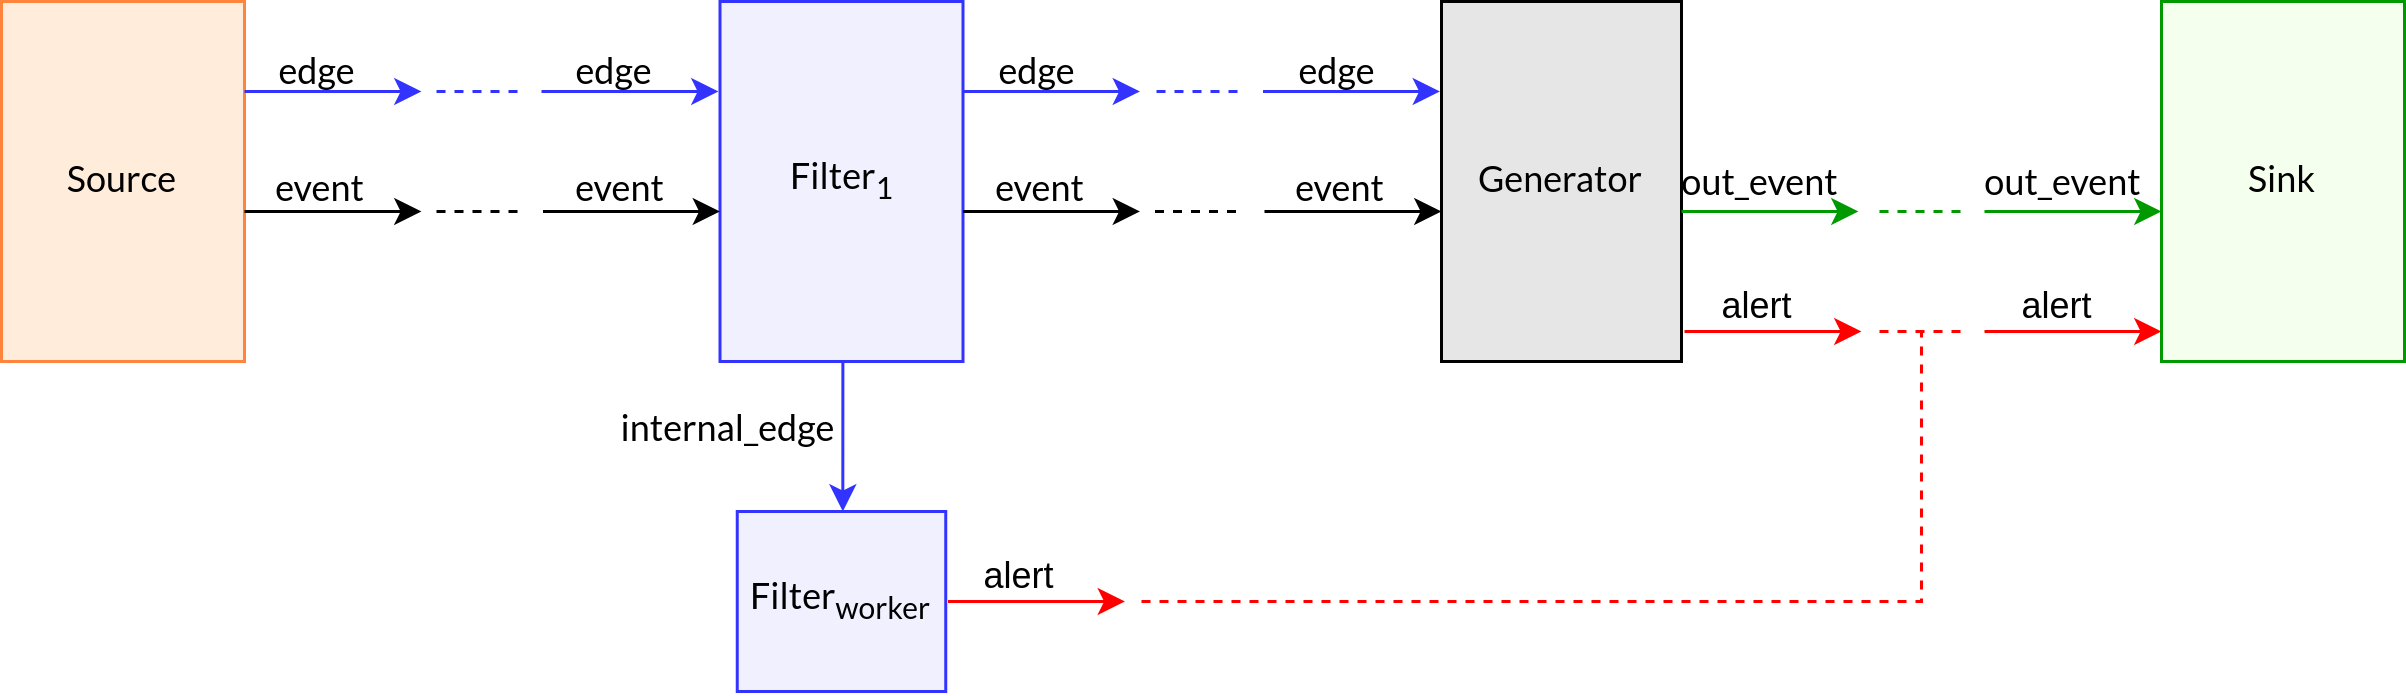
\includegraphics[scale = 0.7]{images/pipeline-schema-filter-detail.png}
  \caption{Pipeline Schema with Filter detail}
  \label{img:pipeline-schema}
\end{figure}


\textcolor{red}{\textbf{Problem detected}\\
If the EOF event is sent through the event channel then it can happen that this event reaches / is treated before the full stream of edges is fully read / processed, leading to
the termination of the processes before the processing of all the edges.\\
Therefore, we decide to merge the edge and the event channel in one single channel!}


Some notes on the implementation decisions:

\subsection{Filter worker}

Options:

\begin{itemize}
  \item External (named) goroutine
  \item \textcolor{green}{$\rightarrow$} Internal anonymous goroutine
\end{itemize}

Advantages of this decision:
\begin{itemize}
  \item Code simplification, the filter worker can access the variables of the scope of the
  filter (no need to pass them as parameters). This is particularly useful in the case of the \texttt{alert} channel, to which the worker is able to write directly. Same in the case of the \texttt{internal\_edge} channel.
\end{itemize}

and in the case of passing the edges of the card from the filter to the filter worker:
\begin{itemize}
  \item Shared buffer using mutex
  \item \textcolor{green}{$\rightarrow$} Channel 
\end{itemize}

In the case of having a shared buffer to communicate the edges between the filter and the worker a mutex is needed. This is because the filter and the worker can possible write and read, respectively, into this buffer at the same time. With it we will avoid race conditions in the sharing of the buffer. However, a channel or other kind of tool would be needed to indicate the worker that there is an edge ready to be read in the buffer. Not having this, would imply to continuosly have the worker requesting the mutex to read from the buffer, even when it is empty and there is no edge to read. 

Therefore as a much more simple alternative, we decided to use an internal channel \texttt{internal\_edge} in between the filter and the worker. With it we avoid having to use a mutex and leading with its derived coordination issues. As a general use case channels are typically used for \emph{passing the ownership of data} which is the case we are dealing with.

Some links:
\begin{itemize}
  \item \href{https://stackoverflow.com/questions/47312029/when-should-you-use-a-mutex-over-a-channel}{When should you use a mutex over a channel?}
  \item \href{https://go.dev/wiki/MutexOrChannel}{Go Wiki - use a mutex or channel?}
\end{itemize}





\begin{figure}[H]
  \centering
  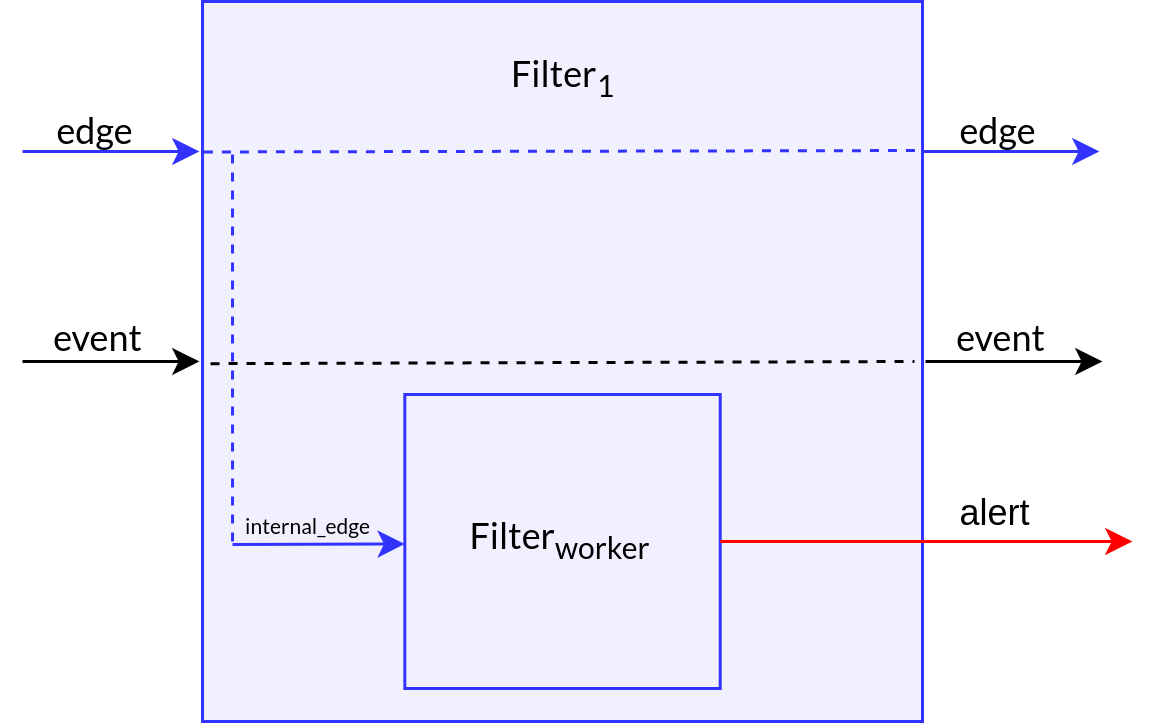
\includegraphics[scale = 0.7]{images/filter-worker.png}
  \caption{Filter Worker detail}
  \label{img:pipeline-schema}
\end{figure}



\section{Fraud Patterns}

\subsection{Fraud Pattern I - Card Cloning}

A first algorithmic proposal to detect this kind of fraud pattern is the one shown in the algorithm
\ref{alg:check-fraud-1}. Note that $S$ refers to the filter's subgraph and $e_{new}$ is the new incoming edge belonging to the filter, such that it is a opening interaction edge, since in the case it is a closing interaction edge, we do not perform the \text{CheckFraud()}.

\begin{algorithm}[H]
    \small
    \begin{algorithmic}[1]
    \REQUIRE $S$ is the subgraph of edges of the filter (sorted by time)
    \REQUIRE $e_{new}$ is the new incoming opening interaction edge belonging to the filter 
    \STATE $\texttt{fraudIndicator} \gets \texttt{False}$
    \STATE $i \gets |S|$
    \WHILE{$i > 0$ \AND \texttt{fraudIndicator} = \texttt{False}}
      \STATE $e_i \gets S[i]$
      \STATE $\texttt{t\_min} \gets \text{obtain\_t\_min}(e_i, e_{new})$
      \STATE $\texttt{t\_diff} \gets e_{new}.start - e_i.end$
      \IF{$\texttt{t\_diff} < \texttt{t\_min}$}   
        \STATE $\text{createAlert}(e_i, e_{new})$
        \STATE $\texttt{fraudIndicator} \gets \texttt{True}$
      \ENDIF
      \STATE $i \gets i - 1$
    \ENDWHILE
    \end{algorithmic}
    \caption{$\text{CheckFraud}(S, e_{new})$ -- \textbf{initial version}}
    \label{alg:check-fraud-1}
\end{algorithm}

There are some aspects and decisions of this algorithm that are worth to describe:

\begin{itemize}
    \item \textbf{Pairwise detection}. The checking of the anomalous fraud scenario is done doing the check between the new incoming edge $e_{new}$ and each of the edges $e_i$ of the filter's subgraph $S$.
    \item \textbf{Backwards order checking}. The pairs $(e_{new}, e_i)$ are checked in a backwards traversal order of the edge list of the subgraph $S$, starting with the most recent edge of the subgraph and ending with the oldest.  
    \item \textbf{Stop the checking whenever the first anomalous scenario is detected}. Whenever an anomalous scenario corresponding to a pair ($e_{new}, e_i)$, then we stop the checking at this point and emit the corresponding alert. Therefore we do not continue the checking with previous edges of $S$. 
    \item \textbf{Emission of the pair $(e_{new}, e_i)$ as the alert}. The alert is composed by the pair $(e_{new}, e_i)$ that is detected to cause the anomalous scenario. Both edges are emitted in the alert since we do not know which is the one that is the anomalous. On the one hand, it can be $e_i$, which is previous to $e_{new}$, in the case that $e_i$ at the moment it arrived it did not cause any alert with the previous edges/transactions of the subgraph and it causes it now with a new incoming edge $e_{new}$ which is a regular transaction of the client. On the other hand, it can be $e_{new}$, which is the last having arrived to the system, that it directly causes the alert with the last (ordinary) transaction of the card.
\end{itemize}

However, a more detailed study, lead us to a simplification of the initially proposed algorithm to the one shown in \ref{alg:check-fraud-def}. On it we just perform the checking between the new incoming edge $e_{new}$ and the most recent edge of the subgraph $S$, $e_{last}$.

\begin{algorithm}[H]
  \small
  \begin{algorithmic}[1]
  \REQUIRE $S$ is the subgraph of edges of the filter (sorted by time)
  \REQUIRE $e_{new}$ is the new incoming opening interaction edge belonging to the filter 
  \STATE $last \gets |S|$
  \STATE $e_{last} \gets S[last]$
  \STATE $\texttt{t\_min} \gets \text{obtain\_t\_min}(e_{last}, e_{new})$
  \STATE $\texttt{t\_diff} \gets e_{new}.start - e_{last}.end$
  \IF{$\texttt{t\_diff} < \texttt{t\_min}$}   
    \STATE $\text{createAlert}(e_{last}, e_{new})$
  \ENDIF
  \end{algorithmic}
  \caption{$\text{CheckFraud}(S, e_{new})$ -- \textbf{definitive version}}
  \label{alg:check-fraud-def}
\end{algorithm}


In what follows we argument the reason why it is sufficient to just check the fraud scenario among $e_{new}$ and the last/most recent edge of the subgraph and not have to continue having to traverse the full list of edges.

Assume that we have a subgraph as depicted in Figure \ref{img:fp-I-demo}, and that we do not know if there have been anomalous scenarios produced between previous pairs of edges of the subgraph. Name $F_I(y_i,y_j)$ a boolean function that is able to say whether it exists an anomalous fraud scenario of this type between the pair of edges $(y_i,y_j)$ or not. In addition, note that the edges of the subgraph $S$ are ordered by time in ascending order, in such a way that $y_1 < y_2 < y_3$. Finally note that $y_3 \equiv e_{new}$ as it is the new incoming edge and $y_2 \equiv e_{last}$, since it is the last edge / the most recent edge of $S$.

\begin{figure}[H]
  \centering
  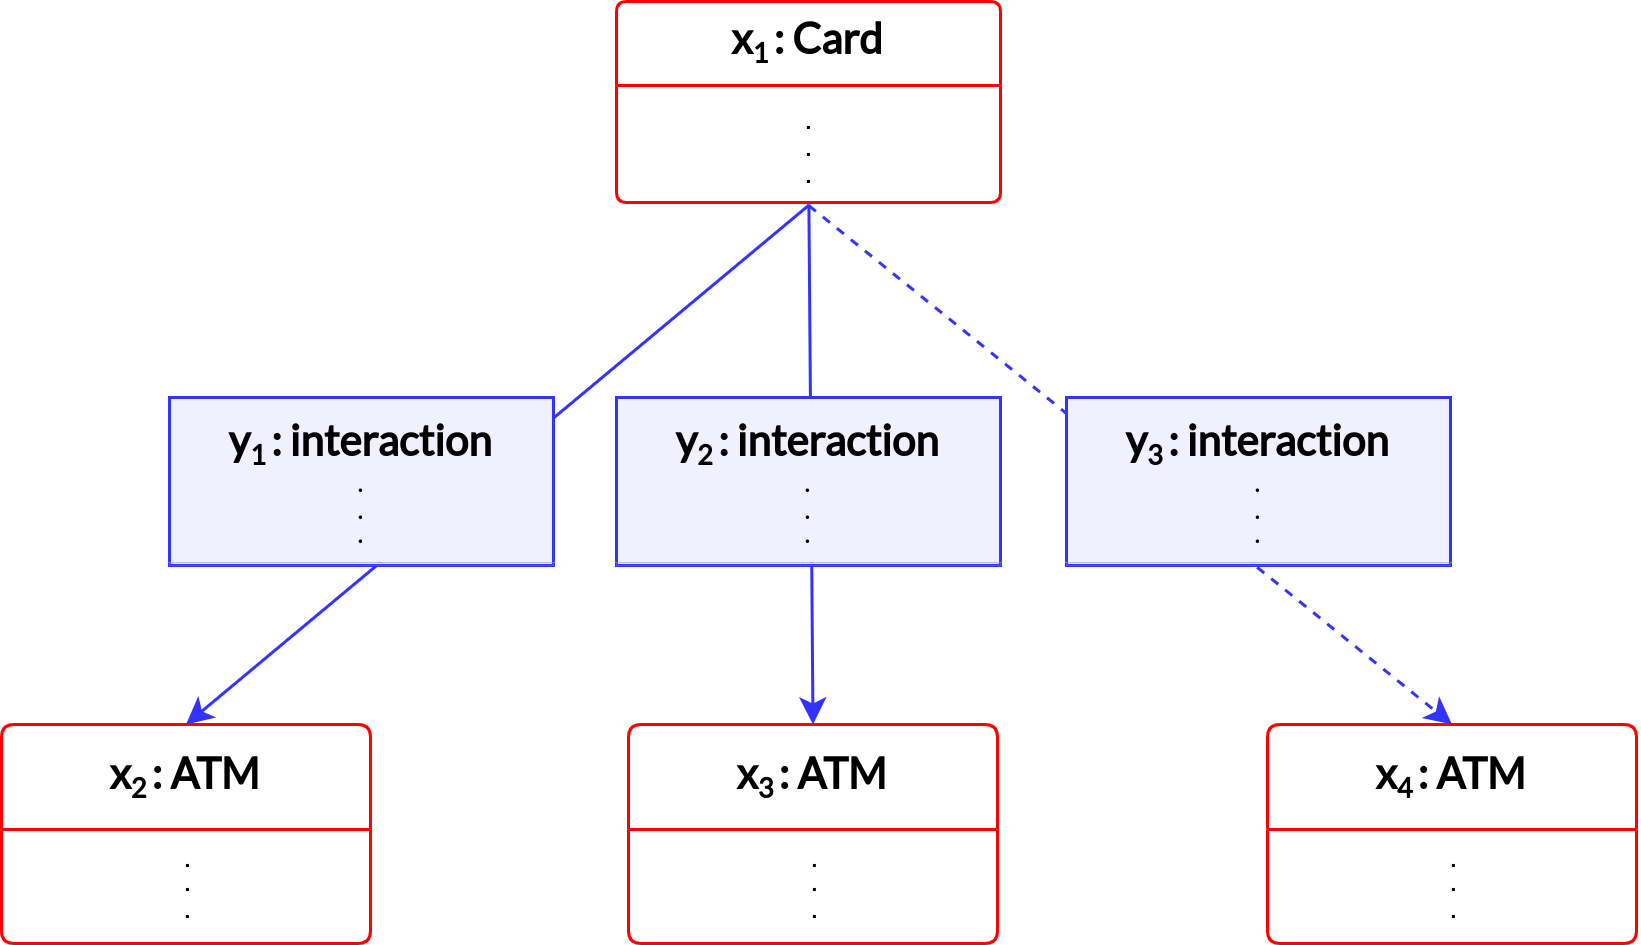
\includegraphics[scale = 0.6]{images/fp-I-demo-1.png}
  \caption{Subgraph $S$ of a card -- Fraud Pattern I}
  \label{img:fp-I-demo}
\end{figure}

Note that we can have that:
\begin{itemize}
    \item $F_I(y_2,y_3)$: We emit an alert of this anomalous scenario produced between the pair $(y_2,y_3)$. We could continue checking for anomalous scenarios between $y_3$ and previous edges of the subgraph. However, what we consider important for the bank system is to detect the occurrence of an anomalous scenario in a certain card. Therefore, we consider that, to achieve this, it is enough to emit a single alert of anomalous scenario on this card, and not many related with the same incoming transaction of the same card.
    \item $\neg F_I(y_2,y_3)$: We analyze whether it would be interesting or not to continue the checking with previous edges of the subgraph, based on assumptions on the fraud checking between previous edges. In particular we can have two cases:
    \begin{itemize}
        \item If $F_I(y_1,y_2)$: Having this it can happen that either $F_I(y_1,y_3)$ or $\neg F_I(y_1,y_3)$. In the case of $F_I(y_1,y_3)$, since $\neg F_I(y_2,y_3)$, we can infer that the anomalous scenario detected between $y_1$ and $y_3$ is a continuation of the same previous anomalous scenario detected between $y_1$ and $y_2$. Therefore, we can conclude that this does not constitute a new anomalous scenario that would require an alert.
        \item If $\neg F_I(y_1,y_2)$: It can be shown that \emph{by transitivity}, having \\
        $\neg F_I(y_1,y_2) \land \neg F_I(y_2,y_3)
        \implies \neg F_I(y_1,y_3)$. \\
        \textcolor{red}{TODO: Show a formal demostration of this case!}
    \end{itemize}
\end{itemize}

Therefore, we have seen that, it is enough to perform the checking between the pair formed by $e_{new}$ and the most recent edge of the subgraph $e_{last}$. $\square$


\textcolor{red}{\rule{\textwidth}{1mm}}
\textcolor{red}{TODO: Complete other aspects of the filter worker algorithmic workflow\\}
Others -- not so much related with the CheckFraud algorithm, but in general with the filter's algorithm --:
\begin{itemize}
    \item Save all the edges in the subgraph $S$, even though they are the reason of the creation of an anomalous scenario.
    \item Number of anomalous fraud scenarios that can be detected. Bounded by:
    $$\#TX\_ANOM \leq SCENARIOS \leq 2*\#TX\_ANOM$$
\end{itemize}


%\bibliographystyle{plain} % Choose a style (plain, abbrv, unsrt, etc.)
%\bibliography{references} % This points to references.bib  

\end{document}